\subsection{Proceso Interno 06: Definir Condiciones}

\subsubsection{Objetivo del Proceso}
Configurar parámetros operativos clave en una simulación REBOUND para:
\begin{itemize}
    \item Establecer condiciones de integración numérica
    \item Definir constantes físicas fundamentales
    \item Preparar simulación para cálculo de LE
\end{itemize}

\subsubsection{Entradas Principales}
\begin{itemize}
    \item \textbf{sim}: Referencia a objeto \texttt{Simulation} configurado
    \item \textbf{sim\_params}: Estructura con:
    \begin{itemize}
        \item $dt \in \mathbb{R}^+$ (paso temporal)
        \item $G \in \mathbb{R}^+$ (constante gravitacional)
        \item $T_{\text{max}} \in \mathbb{R}^+$ (tiempo máximo)
    \end{itemize}
\end{itemize}

\subsubsection{Sub-pasos Secuenciales}
Este apartado es proporcionado para profundizar y describir de forma textual cada paso contenido dentro del diagrama del proceso descrito en la figura~\ref{fig:process_diagram06}
\subsubsection*{1. Recibir Instancia y Parámetros}
\begin{itemize}
    \item Capturar \texttt{sim} y \texttt{sim\_params}
\end{itemize}

\subsubsection*{2. Desempaquetar Parámetros}
\begin{itemize}
    \item Extraer: $dt, G, T_{\text{max}}$
\end{itemize}

\subsubsection*{3. Validación Opcional}
\begin{equation*}
    \begin{cases}
    dt > 0 \\
    G > 0 \\
    T_{\text{max}} > \texttt{sim.t} \\
    \end{cases}
\end{equation*}

\subsubsection*{4. Establecer Parámetros en REBOUND}
\begin{verbatim}
sim.dt = dt  # Paso temporal
sim.G = G    # Constante gravitacional
\end{verbatim}

\subsubsection*{5. Procesar Tiempo Máximo}
\begin{itemize}
    \item Almacenar $T_{\text{max}}$ para control externo
    \item No modifica estado interno de \texttt{sim}
\end{itemize}

\subsubsection*{6. Verificación de Compatibilidad}
\begin{itemize}
    \item Chequear coherencia integrador/parámetros
    \item Ejemplo: $\texttt{sim.integrador} == \texttt{IAS15}$
\end{itemize}

\subsubsection{Lógica Interna y Decisiones}
\begin{itemize}
    \item \textbf{Validaciones}:
    \begin{itemize}
        \item Condicionales según política del sistema
        \item Manejo de errores por valores inválidos
    \end{itemize}
    \item \textbf{Compatibilidad}:
    \begin{itemize}
        \item Verificación implícita de estabilidad numérica
    \end{itemize}
\end{itemize}

\subsubsection{Manejo de Datos Específico}
\begin{itemize}
    \item \textbf{Entradas}:
    \begin{itemize}
        \item Parámetros de configuración temporal/física
        \item Instancia REBOUND preconfigurada
    \end{itemize}
    \item \textbf{Intermedios}:
    \begin{itemize}
        \item Estado modificado de \texttt{sim}
        \item $T_{\text{max}}$ almacenado para ejecución
    \end{itemize}
    \item \textbf{Salida}:
    \begin{itemize}
        \item Simulación lista para ejecución
        \item $T_{\text{max}}$ disponible como metadato
    \end{itemize}
\end{itemize}

\subsubsection{Salidas Principales}
\begin{itemize}
    \item \texttt{sim} configurado con:
    \begin{itemize}
        \item $dt$ para integración numérica
        \item $G$ para interacciones gravitatorias
    \end{itemize}
    \item $T_{\text{max}}$ como parámetro de control
\end{itemize}

\subsubsection{Interacciones Internas}
\begin{itemize}
    \item \textbf{Con API REBOUND}:
    \begin{itemize}
        \item Modificación directa de propiedades \texttt{sim}
        \item Consulta de estado del integrador
    \end{itemize}
    \item \textbf{Con flujo de control}:
    \begin{itemize}
        \item Transmisión de $T_{\text{max}}$ a siguiente etapa
    \end{itemize}
\end{itemize}
\newpage
\subsubsection{Diagrama del Proceso}
\begin{figure}[H]
    \centering
    \adjustbox{max width=\textwidth, max height=0.9\textheight}{%
        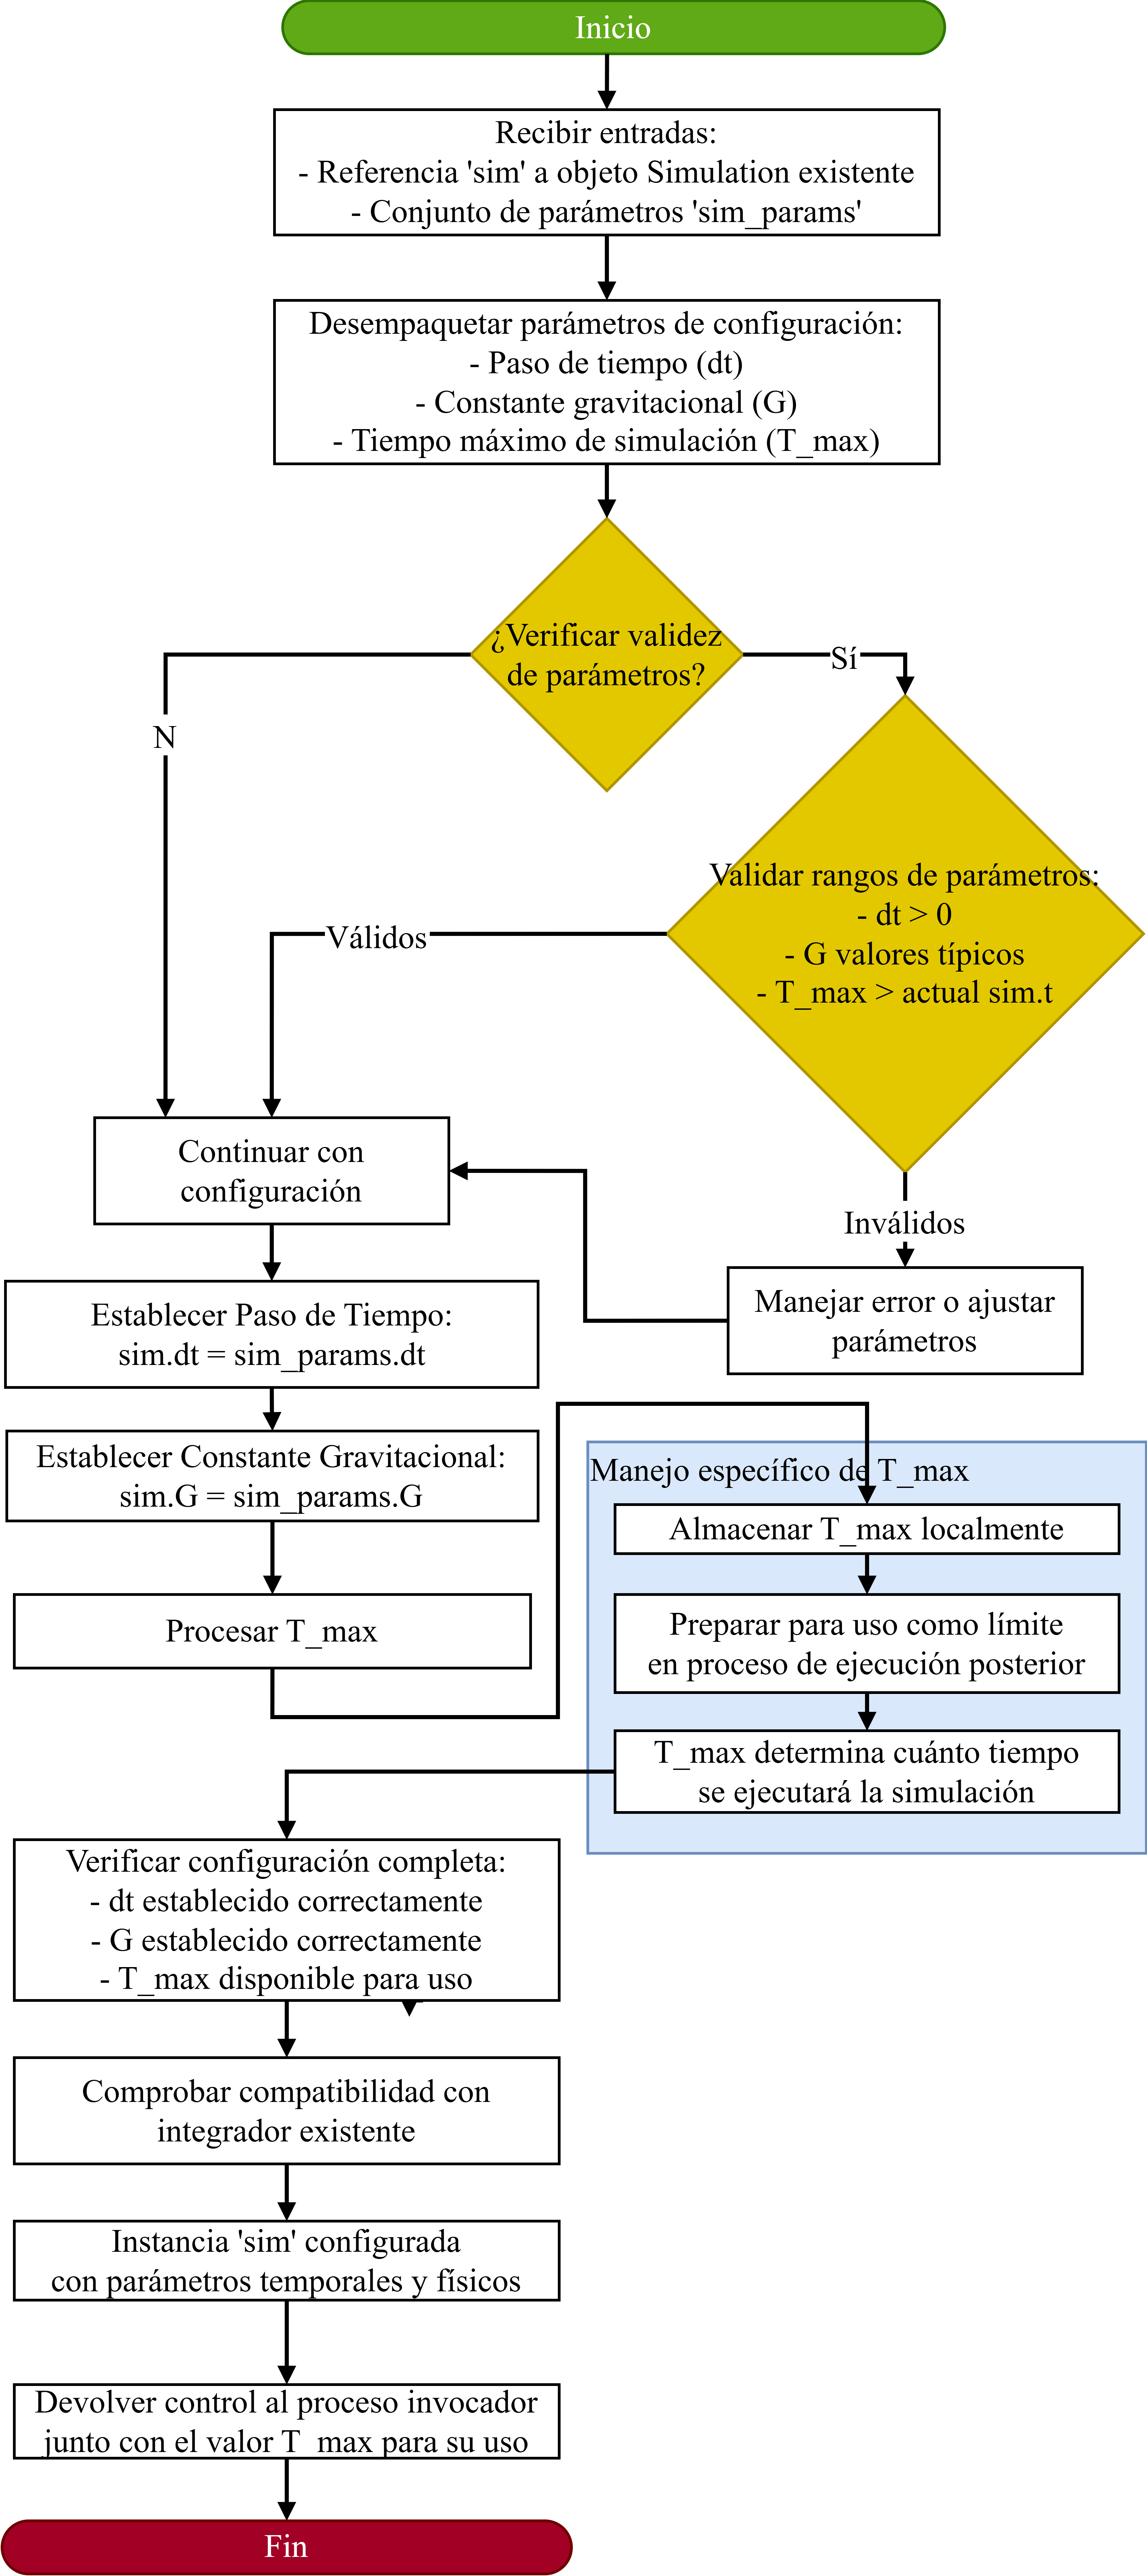
\includegraphics{img/Analisis/DiagramaProcesos/DiagramaProceso06_DefinirCondiciones.png}
    }
        \caption{Diagrama de Proceso Interno 06: Definir Condiciones}%
    \label{fig:process_diagram06}
\end{figure}
\newpage